%Aufgabenteil a)
\subsection{Temperaturmessung}
Im folgenden Diagramm werden die Verläufe der Temperaturen T1 und T2 in Abhängigkeit der Zeit aufgetragen.
Alle Werte wurden in SI-Einheiten konvertiert.
\begin{figure}
  \centering
  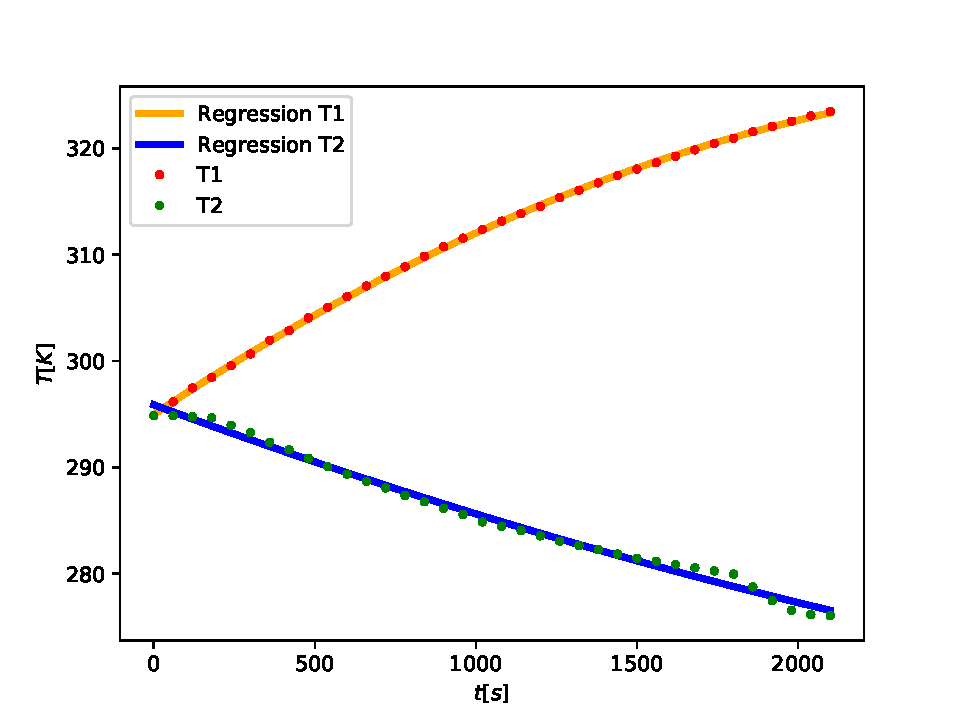
\includegraphics[scale = 0.75]{Temperaturverlaeufe.pdf}
  \caption{Die beiden Temperaturverläufe der Reservoire 1 und 2.}
  \label{fig:TemperaturverlaufA}
\end{figure}

%Aufgabenteil b)
\subsection{Bestimmung der Näherungsfunktion}
Die quadratische Regression ist ebenfalls in Abbildung \ref{fig:TemperaturverlaufA} skizziert. Der gewählte Ansatz ist
\begin{equation}
  T(t) = \symup{A} \cdot t^2 + \symup{B} \cdot t + \symup{C}.
  \label{eq:Regressionsgleichung}
\end{equation}
\begin{table}
  \centering
  \caption{Parameter der quadratischen Regression}
  \label{tab:regression1}
  \sisetup{table-format=3.7}
  \begin{tabular}{c S S S S S S}
    \toprule
     {$T$} & {$A [\mu K/s^2]$} & {$\increment A [nK/s^2]$} & {$B [mK/s]$} & {$\increment B [\mu K/s]$} & {$C [K]$} & {$\increment C [K]$} \\
    \midrule
    {$T_\text{1}$} & -3.22492 &  41.934 &  20.27984 & 91.1047 & 294.97008 & 0.04134 \\
    {$T_\text{2}$} & 0.95504 &  267.11 & -11.20871 & 580.316 & 295.87019 & 0.26336 \\
    \bottomrule
  \end{tabular}
\end{table}

%Aufgabenteil c)
\subsection{Bestimmung der Differentialquotienten}
Die Differentialquotienten der Regressionen berechnet man durch einfaches Ableiten der Gleichung \eqref{eq:Regressionsgleichung}.
Nach den Ableitungsregeln ergibt sich:
\begin{equation}
    T'(t) = 2\symup{A} \cdot t + \symup{B}
    \label{eq:Regressionableitung}
\end{equation}
  Nun werden konkrete Werte für 4 verschiedene Temperaturen berechnet werden. Diese sind in unserem Fall die Temperaturen bei
  den Zeiten $60s, 660s, 1 260s, 1 860s$.
  \begin{table}
    \centering
    \caption{Differentialquotienten}
    \label{tab:Differentialquotienten}
    \sisetup{table-format=1.5}
    \begin{tabular}{c S S S S S S}
      \toprule
       {$t [s]$} & {$T_{1}'(t) [K/s]$} & {$\increment T_{1}'(t) [\mu K/s]$} & {$T_{2}'(t) [K/s]$} & {$\increment T_{2}'(t) [mK/s]$} \\
      \midrule
      60 & 0.02027 & 91.1047 & 0.01121 & 0.580316 \\
      660 & 0.02020 & 91.1047 & 0.01118 & 0.580345 \\
      1260 & 0.02014 & 91.1216 & 0.01117 & 0.580424 \\
      1860 & 0.02007 & 91.1417 & 0.01115 & 0.580552 \\
      \bottomrule
    \end{tabular}
  \end{table}

\subsection{Bestimmung der Güteziffer}
Mithilfe der Differentialquotienten soll mit \eqref{eqn:realegüteziffer3} die reale Güteziffer berechnet werden. Zudem soll diese mit der
idealen Güteziffer verglichen werden, die mit \eqref{eqn:idealegüteziffer} berechnet wird.
Die Abweichung p der Beiden Werte in Prozent wird berechnet mit:
\begin{equation}
  p=\frac{v_{id}-v_{real}}{v_{id}} \cdot 100
\end{equation}
Die Berechnung bei den vier oben beschriebenen
Zeitpunkten ergibt:
\begin{table}
  \centering
  \caption{Güteziffern für T1}
  \label{tab:gütezifferT1}
  \sisetup{table-format=1.5}
  \begin{tabular}{S[table-format=4.1] S S S[table-format=3.0] S[table-format=2.5] S}
    \toprule
    {$t [s]$} & {$v_{real1}$} & {$\increment v_{real1}$} & {$v_{id1}$} & {$p_1$} & {$\increment p_1$} \\
    \midrule
    60 & 2.95349 & 0.01327 & 227 & 98.70351 & 0.00583 \\
    660 & 2.94409 & 0.01327 & 16 & 82.35746 & 0.07954 \\
    1260 & 2.93470 & 0.01327 & 9 & 69.94106 & 0.13597 \\
    1860 & 2.87735 & 0.01306 & 7 & 61.70096 & 0.17384 \\
      \bottomrule
  \end{tabular}
\end{table}

\begin{table}
\centering
\centering
  \caption{Güteziffern für T2}
  \label{tab:gütezifferT2}
  \sisetup{table-format=1.5}
  \begin{tabular}{S[table-format=4.0] S S S[table-format=3.0] S[table-format=2.5] S}
    \toprule
     {$t [s]$} & {$v_{real2}$} & {$\increment v_{real2}$} & {$v_{id2}$} & {$p_2$} & {$\increment p_2$} \\
    \midrule
    60 & 1.63264 & 0.08454 & 226 & 99.28016 & 0.03727 \\
    660 & 1.62986 & 0.08454 & 15 & 89.61044 & 0.53894 \\
    1260 & 1.62707 & 0.08456 & 8 & 69.94105 & 0.96492 \\
    1860 & 1.59767 & 0.08319 & 6 & 75.46897 & 1.27773 \\
      \bottomrule
  \end{tabular}
\end{table}

Es fällt auf, dass die Abweichung der realen Güteziffer von dem idealen Wert stark abweicht.
Mögliche Gründe für diese Abweichung werden in \ref{sec:Auswertung} angegeben.

\subsection{Bestimmung des Massendurchsatzes}
Die Berechnung des Massendurchsatzes erfolgt mit \eqref{eqn:massendurchsatz2}. Dafür muss aber zuerst die
Verdampfungswärme L bestimmt werden.
\\
Aus V203 (Verdampfungswärme) ist folgender Zusammenhang zwischen dem Druck p, der Temperatur T, und L bekannt:
\begin{equation}
  ln(p/p_0)=\frac{-L}{R \cdot T}
\end{equation}
$R$ entspricht hierbei der universellen Gaskonstante und $p_0$ entspricht der Umgebungsdruck.
Wählt man nun $x=1/T$ und $y=ln(p-p_0)$, dann erhält man die lineare Gleichung:
\begin{equation}
  y=-\frac{L}{R}\cdot x+c \label{Dampfdruckgleichung}
\end{equation}
Trägt man die Messwerte in ein Koordinaten System ein und setzt wie oben beschrieben $x=1/T$ und $y=ln(p-p_0)$,
wird dieser Zusammenhang gut ersichtlich.
\begin{figure}
  \centering
  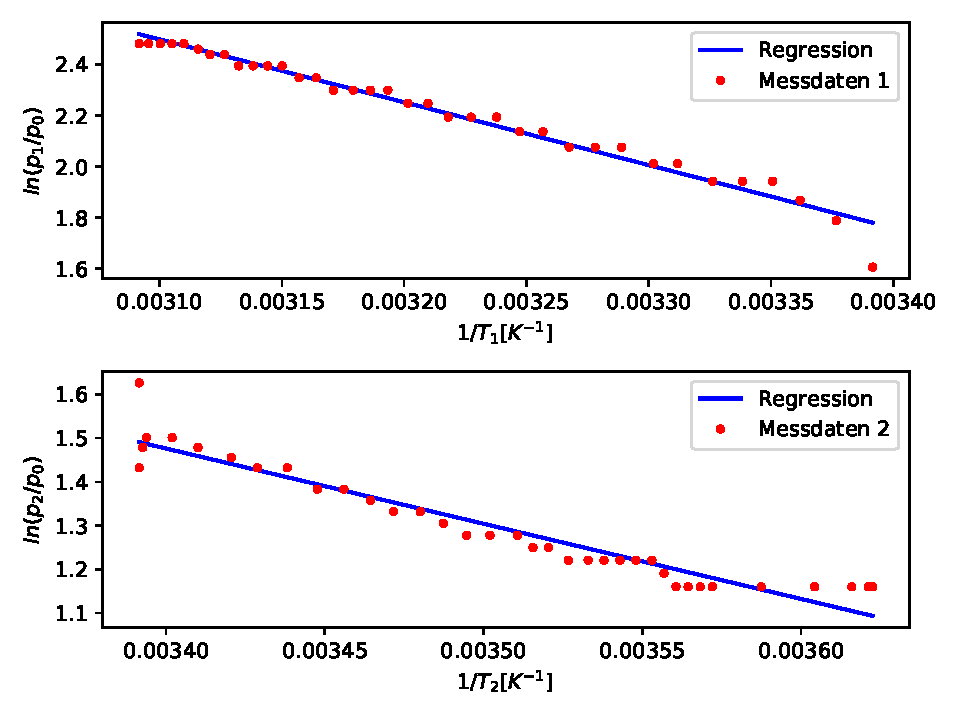
\includegraphics[scale = 0.75]{Druckverlaeufe.pdf}
  \caption{Dampfdruckkurve}
  \label{fig:Dampfdruckkurve}
\end{figure}
Die eingezeichnete Regression hat nun genau die Funktionsgleichung \eqref{Dampfdruckgleichung}. Die Steigung der
Gerade ist demnach $m=-L/R$. L erhält also durch $L=-m\cdot R$. Durch Einsetzen folgt:
\\
$L=\SI{14299.459 \pm 734.742}{\joule\second\kelvin\per\mole}$
\\
Mit \eqref{eqn:massendurchsatz2} kann man jetzt für die vier verschiedenen Zeiten den Massendurchsatz errechnen:
\begin{table}
  \centering
  \caption{Massendurchsatz}
  \label{tab:massendurchsatz}
  \sisetup{table-format=1.5}
  \begin{tabular}{S[table-format=4.0] S S S S}
    \toprule
    {$t [s]$} & {$\frac{dm}{dt} [mol/s]$} & {$\increment\frac{dm}{dt}[mol/s]$} & {$\frac{dm}{dt} [g/s]$} & {$\increment\frac{dm}{dt}[g/s]$} \\
    \midrule
    60 & 0.01370 & 0.00100 & 1.65659 & 0.12084 \\
    660 & 0.01365 & 0.00100 & 1.65377 & 0.12075 \\
    1 260 & 0.01365 & 0.00100 & 1.65095 & 0.12065 \\
    1 860 & 0.01363 & 0.00100 & 1.64812 & 0.12057 \\
    \bottomrule
  \end{tabular}
\end{table}
Der Massendurchsatz wird in \ref{tab:massendurchsatz} sowohl in $\si{\mole\per\second}$, als auch in $\si{\gram\per\second}$ angegeben.
Man erreicht die Umrechnung mit:
\begin{equation}
  m=M\cdot n
\end{equation}
Hierbei ist $M$ die Molmasse des Gases Dichlordifluormethan $M_{CCl_{2}F_{2}}=\SIlist{120.9}{\kilogram\per\mole}$.

\subsection{Bestimmung der mechanischen Kompressorleistung}
Die mechanische Kompressorleistung $N_{mech}$ wird mit \eqref{eqn:leistungkompressor2} berechnet.
Dabei gilt:
\begin{equation}
  \frac{dV_2}{dt}=\frac{1}{\rho}\frac{dm}{dt} \label{Volumenänderung}
\end{equation}
Das $\rho$ hierbei die Dichte des Gases in Abhängigkeit der Temperatur und des Drucks.
Die Dichte kann man nun mit dem idealen Gasgesetz
\begin{equation}
  pV=nRT \Leftrightarrow \frac{pV}{T}=nR
\end{equation}
berechnen. Da die Stoffmenge $n$ des Gases immer konstant ist, da kein Gas entweicht oder zugeführt wird, und auch
$R$ eine Konstante ist, ist die ganze rechte Seite konstant. Diese Seite ist für die Temperatur $T_2$, den Druck $p_2$ und das
Volumen $V_2$ gleich den Werten, bei denen die Dichte $\rho_0=\SI{5.514}{\gram\per\liter}$ des Gases gemessen wurde. Diese lauten
$p_0=\SI{e5}{\pascal}$ und $T_0=\SI{273.15}{\kelvin}$.
\begin{equation}
  \frac{p_2V_2}{T_2}=\frac{p_0V_0}{T_0} \Leftrightarrow \frac{p_2m}{\rho_2T_2}=\frac{p_0m}{\rho_0T_0}
\end{equation}
Da die auch die Masse des Gases konstant ist, kann diese gekürzt werden.
Umstellen nach $\rho_2=\rho$ ergibt:
\begin{equation}
  \rho=\frac{\rho_0T_0p_1}{T_2p_0} \label{rho}
\end{equation}
\\
Mit \eqref{rho} und \eqref{Volumenänderung} kann \eqref{eqn:leistungkompressor2} geschrieben werden als:
\begin{equation}
  N_\text{mech} = \frac{1}{\kappa - 1}  \left(p_\text{b} \sqrt[\kappa]{\frac{p_\text{a}}{p_\text{b}}} - p_\text{a} \right)
  \frac{T_2p_0}{\rho_0T_0p_a}\frac{dm}{dt}
\end{equation}
Die mechanische Leistung des Kompressors ist nach Einsetzen der vier ausgewählten Zeiten:
\begin{table}
  \centering
  \caption{mechanische Kompressorleistung}
  \label{tab:kompressorleistung}
  \sisetup{table-format=1.5}
\begin{tabular}{S[table-format=4.0] S[table-format=2.5] S S[table-format=2.5] S}
  \toprule
  {$t [s]$} & {$N_\text{mech} [W]$} & {$\increment N_\text{mech} [W]$} & {$\rho [kg/m^3]$} & {$\increment\rho [kg/m^3]$} \\
  \midrule
  60 & 18.02604 & 0.92977 & 30.53529 & 0.01356\\
  660 & 37.45139 & 1.93178 & 44.18748 & 0.01530\\
  1 260 & 49.78378 & 2.56797 & 53.01378 & 0.01873\\
  1 860 & 59.01109 & 3.04402 & 64.59788 & 0.02317\\
  \bottomrule
\end{tabular}
\end{table}
